\documentclass[twoside]{article}

\usepackage[math]{kurier}
\usepackage[sc]{mathpazo}
\renewcommand{\sfdefault}{kurier}

\usepackage[boxruled]{algorithm2e}
\usepackage[utf8]{inputenc}
\usepackage[backend=biber]{biblatex}
\usepackage[english]{babel}
\usepackage[english]{babel}
\usepackage[autostyle]{csquotes}
\usepackage{placeins}
\usepackage[backend=biber]{biblatex}
\bibliography{./lecture_17_biblio.bib}

\usepackage{graphics}
\usepackage{graphicx}
\usepackage{subcaption}
\usepackage{amsmath}
\usepackage{float}
\setlength{\oddsidemargin}{0.25 in}
\setlength{\evensidemargin}{-0.25 in}
\setlength{\topmargin}{-0.6 in}
\setlength{\textwidth}{6.5 in}
\setlength{\textheight}{8.5 in}
\setlength{\headsep}{0.75 in}
\setlength{\parindent}{0 in}
\setlength{\parskip}{0.1 in}


\newcounter{lecnum}
\renewcommand{\thepage}{\thelecnum-\arabic{page}}
\renewcommand{\thesection}{\thelecnum.\arabic{section}}
\renewcommand{\theequation}{\thelecnum.\arabic{equation}}
\renewcommand{\thefigure}{\thelecnum.\arabic{figure}}
\renewcommand{\thetable}{\thelecnum.\arabic{table}}


\newcommand{\lecture}[3]{
   \pagestyle{myheadings}
   \thispagestyle{plain}
   \newpage
   \setcounter{lecnum}{#1}
   \setcounter{page}{1}
   \noindent
   \begin{center}
   \framebox{
      \vbox{\vspace{2mm}
    \hbox to 6.28in { {\bf \sffamily AA 274: Principles of Robotic Autonomy
                        \hfill Winter 2019} }
       \vspace{4mm}
       \hbox to 6.28in { {\sffamily{\Large \hfill Lecture #1: #2  \hfill}} }
       \vspace{2mm}
       % \hbox to 6.28in { {\it \hfill Scribes: #4} }
      \vspace{2mm}}
   }
   \end{center}
   \markboth{Lecture #1: #2}{Lecture #1: #2}

   \vspace*{4mm}
}


%%%%%%%%%%%%%%%%%%%%%%%%%%
%document
\begin{document}
%modify this
\lecture{17}{Decision Making and Dynamic Programming}{}

\section{Introduction}
The objective of this lecture is to introduce concepts related to decision making under uncertainty, which refers to optimization at the level of task. For an autonomous vehicle such task-level decisions determine whether the vehicle should turn right or left, or what cars should be given priority. This lecture then highlights, given a decision making problem, how to generate feasible models, represent objective cost functions, identify constrains, and apply corresponding algorithms.  

Core learning objectives of the lecture:
\begin{itemize}
    \item Principal of Optimality
    \item Dynamic Programming (DP) Algorithm and Approximation
    \item Certainty Equivalent Control
    \item Cost-to-Go Approximation (CGA)
\end{itemize}

\section{Basic Decision Making Problem}
For decision making in a probabilistic setting, we begin with a discrete model to determine how the system will evolve over time: 

\begin{equation*}
  x_{k+1}=f_{k}\left(x_{k}, u_{k}, w_{k}\right), k=0, \ldots, N
\end{equation*}

where the state at time $k+1$, is a function of the previous state $x_{k}$, control $u_{k}$, and a random disturbance $w _{k}$. Note that this function can be non-linear and the state can include a wide array of information including the charge of the robot or the communication bandwidth.

In this model the control constraints ensure that the controls at time $k$ are chosen from a set which is a function of the state of the robot at time $k$:

\begin{equation*}
    u_{k} \in U\left(x_{k}\right)
\end{equation*}

We also assume that the probability distribution of the disturbance is known and that it is conditional on the current state and the current control: 

\begin{equation*}
    P_{k}(.|x_{k}, u_{k}) \text { of } w_{k}
\end{equation*}

This assumption, which is referred to as the Markov assumption, is made for computational tractability. However, in certain scenarios it may be necessary to model the disturbance as a function of the collection of previous states and controls up to that instance in time. In such cases, we can augment the current state space with the previous states, in order to convert such history-dependent problem to a history-independent one.

Due to uncertainty in a stochastic setting, we cannot operate based on a deterministic future. Therefore we need a closed-loop policy that can map states to controls:

\begin{equation*}
    \pi=\left\{\mu_{0}, \ldots, \mu_{N-1}\right\}, \text { where } u_{k}=\mu_{k}\left(x_{k}\right)
\end{equation*} 

The next component of modeling a decision making problem is defining an additive cost: 

\begin{equation*}
    J_{\pi}\left(x_{0}\right)=E\left\{g_{N}\left(x_{N}\right)+\sum_{k=1}^{N-1} g_{k}\left(x_{k}, \mu_{k}\left(x_{k}\right), w_{k}\right)\right\}
\end{equation*}

This cost includes the terminal cost $g_{N}$ at the final state $X_{N}$ when the robot operations end, and the summation of the stage-wise cost $g_{k}$. Note that $g_{k}$ is a random variable as it is a function of the random disturbance at each stage. To be able to optimize the cost, we then find the expected value of the summation of these random variables. Also note that the expected cost function is additive both in terms of the summation of the stage-wise costs, as well as the additive nature of the expectation function.  

The decision making problem is to optimize over all closed-loop policies to find the one that minimizes the expected cost:  
\begin{equation*}
    J^{*}\left(x_{0}\right)=\min_{\pi} J_{\pi}\left(x_{0}\right)
\end{equation*}

Key points:
\begin{itemize}
    \item Discrete-time model: Could consider continuous-time model, but in most applications the discrete-time is most natural
    \item Markovian model
    \item Objective: find optimal closed-loop policy
    \item Additive cost: central assumption to prove the principle of optimality
    \item Risk-neutral formulation: we only care about expectation and not about variability
\end{itemize}

\section{Principle of Optimality}
The principle of optimality is a key concept that makes stochastic optimal control problem tractable from a computational standpoint. First consider the simplest deterministic case with no stochasticity. Suppose the optimal path for a multistage decision-making problem is shown in the figure below, where the first decision yields segment a-b with cost $J_{ab}$, and remaining decisions yield segments b-e with cost $J_{be}$. The total optimal cost is then $J_{ae}^* = J_{ab} + J_{be}$.

\begin{figure}[!htb]
  \centering
  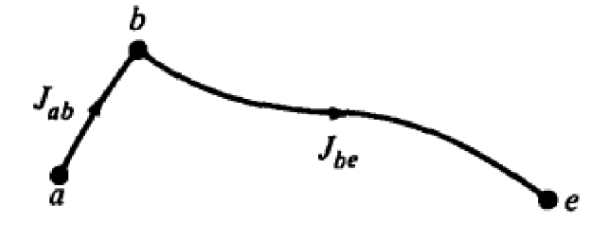
\includegraphics[scale=0.6]{path.PNG}
\end{figure}

The claim of the principle of optimality is as follows: if a-b-e is an optimal path from a to e, then b-e is an optimal path from b to e.

Proof by contradiction: \\
Suppose b-c-e is the optimal path from b to e. Then

\begin{equation*}
    J_{bce} < J_{be}
\end{equation*}

and

\begin{equation*}
    J_{ab} + J_{bce} < J_{ab} + J_{be} = J_{ae}^*
\end{equation*}

\begin{figure}[!htb]
  \centering
  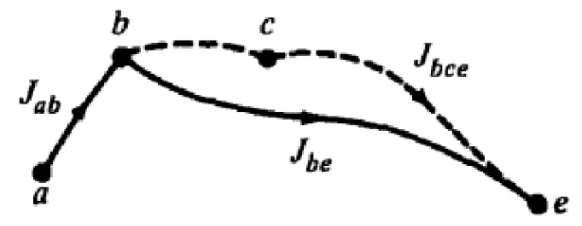
\includegraphics[scale=0.6]{path1.PNG}
\end{figure}

This is a contradiction because $J_{ae}$ is already defined as the optimal path from a to e. If $J_{bce}$ was the optimal path from b to e instead of $J_{be}$, then that would imply that $J_{ae}$ is not optimal. Therefore, $J_{be}$ must be the optimal path from b to e.

\textbf{Remark:} While the principle of optimality holds for tails of optimal policies, the same is not true for heads of optimal policies. Consider a simple game where there are two strategies $\pi_1$, $\pi_2$. The costs as a function of time for these strategies are

\begin{equation*}
    r_1(t) = 10t
\end{equation*}

\begin{equation*}
    r_2(t) = e^{0.1t}
\end{equation*}

and the goal of the game is to accumulate as much reward as possible for the duration of the game.

$$ \pi_{T}^{*}=\arg \min _{i \in\{1,2\}} \sum_{t=1}^{T} r_{i}(t) $$

It is easy to check that if T = 5 the optimal policy is $\pi_2$, and if T = 1000 the optimal policy is $\pi_1$. However, the behavior of $\pi_{1000}^*$ during the first 5 time steps is not the same as the behavior of $\pi_{5}^*$.

\subsection{Definition (for discrete-time systems)}
Let $f^{*} :=\left\{f_{0}^{*}, f_{1}^{*}, \ldots, f_{N-1}\right\}$ be an optimal policy. Assume state $x_k$ is reachable. Consider the subproblem whereby we are at $x_k$ at time $k$ and we wish to minimize the cost-to-go from time $k$ to time $N$. Then, the truncated policy $\left\{f_{k}^{*}, f_{k+1}^{*}, \dots, f_{N-1}^{*}\right\}$ is optimal for the subproblem.

Considering this definition, tail policies are optimal for tail subproblems. Also, mind that the time-dependence is implicit in the notation: $f_k^{*} ( x_k ) = f^{*}(x_k ,k )$.

\subsection{Applying the principle of optimality}
Consider the problem shown in the figure below.

\begin{figure}[!htb]
  \centering
  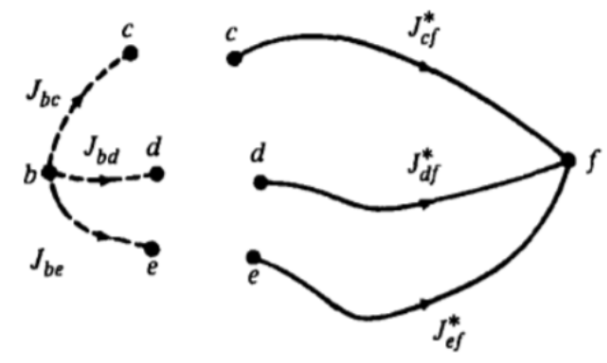
\includegraphics[scale=0.6]{path2.PNG}
\end{figure}

According to the principle of optimality, if b-c is the initial segment of the optimal path from b to f, then c-f is the terminal segment of this path. Hence, the optimal trajectory is found by comparing the following:

$$ C_{b c f}=J_{b c}+J_{c f}^{*}$$
$$  C_{h d f}=J_{b d}+J_{d f}^{*} $$
$$ C_{b e f}=J_{b e}+J_{e f}^{*}$$

The comparison of these three trajectories is shown in the figure below.

\begin{figure}[!htb]
  \centering
  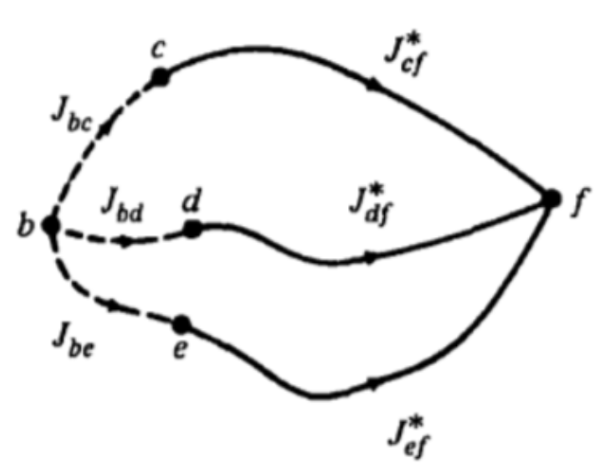
\includegraphics[scale=0.6]{path3.PNG}
\end{figure}

When applying the principle of optimality, one only needs to compare the concatenations of immediate decisions and optimal decisions. This provides a significant decrease in the computation required to solve the problem, and also the amount of possible solutions.

In practice, the principle of optimality is applied \textit{backward} in time. As Soren Kierkegaard said ``Life can only be understood backwards; but it must be lived forwards.”

\subsection{Example Problem}
As an example of solving a problem with the principle of optimality, consider the figure below. The goal is to start from node a and end at node h while incurring the minimum cost along the path. Consider the following movement map: [North: UP], [South: DOWN], [East: RIGHT], [West: LEFT].

\begin{figure}[!htb]
  \centering
  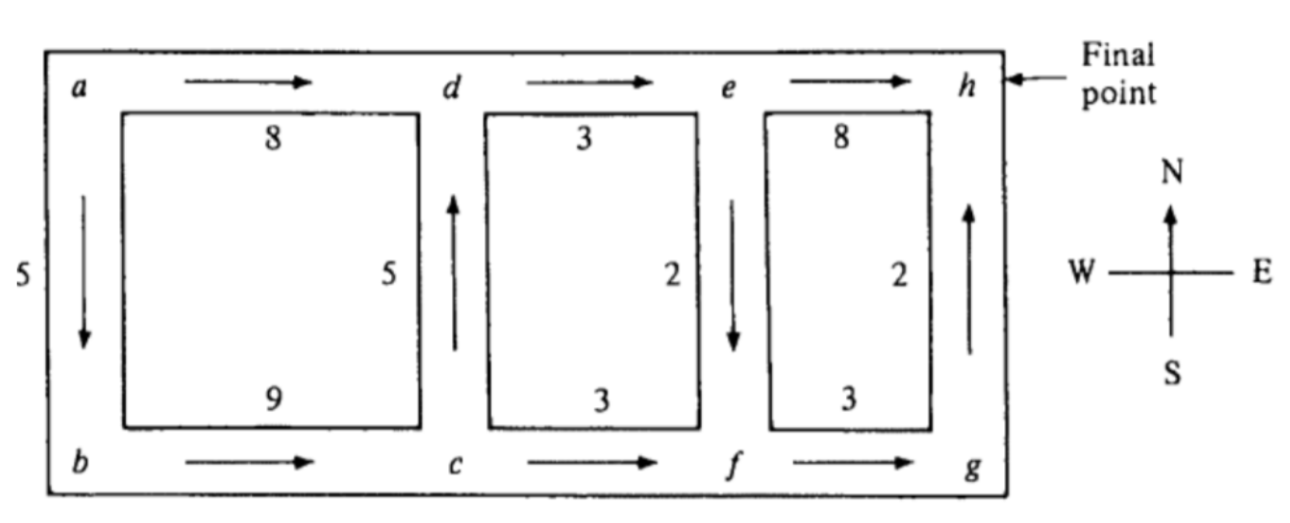
\includegraphics[scale=0.6]{map.PNG}
\end{figure}

As mentioned earlier, in practice, the principle of optimality is applied backward in time. First, consider the cost-to-go from starting at node $h: J(h) = 0$. Then, consider the cost-to-go and optimal action for node $g: J(g) = 2 + J(h) = 2 + 0 = 2, u*(g) = UP$. Continuing for the rest of the problem, we have the following:

$$ 
\begin{aligned} J(f) &=3+J(g)=3+2=5 \\ u^{*}(f) &=R I G H T 
\\ J(e) &=\min (8+J(h)=8,2+J(f)=7)=7 \\ u^{*}(e) &=D O W N 
\\J(d) &=3+J(e)=10 \\ u^{*}(d) &=R I G H T 
\\ J(c) &=\min (5+J(d)=15,3+J(f)=8)=8 \\ u^{*}(c) &=R I G H T
\\ J(b) &=9+J(c)=17 \\ u^{*}(b) &=R I G H T 
\\ J(a) &=\min (5+J(b)=22,8+J(d)=18)=18 \\ u^{*}(a) &=R I G H T \end{aligned}
 $$
 
Thus, the optimal path for this problem is $a \rightarrow d \rightarrow e \rightarrow f \rightarrow g \rightarrow h$. The optimal cost associated with
this path is $J(a) = 18$.

\section{Dynamic Programming (DP) Algorithm}
Model:

$$ 
\boldsymbol{x}_{k+1}=\boldsymbol{a}\left(\boldsymbol{x}_{k}, \boldsymbol{u}_{k}, k\right)
 $$

Cost:

$$ 
J_{f}\left(\boldsymbol{x}_{0}\right)=h_{N}\left(\boldsymbol{x}_{N}\right)+\sum_{k=0}^{N-1} g\left(\boldsymbol{x}_{k}, \boldsymbol{f}_{k}\left(\boldsymbol{x}_{k}\right), k\right)
 $$

Where:
\begin{itemize}
    \item $\boldsymbol{x}_k$ state at time $k$
    \item $\boldsymbol{u}_k$ action at time $k$
    \item $\boldsymbol{a}()$ function which tells us what state to go to given where we are and what we did
    \item $g()$ function which tells us cost of the transition
    \item $h_N(\boldsymbol{x}_N)$ function which tells us the cost of finishing in state $\boldsymbol{x}_N$
    \item $\boldsymbol{f}_k(\boldsymbol{x}_k)$ is the policy function which tells us what to do in state $\boldsymbol{x}_N$
    \item $J_k\boldsymbol{x}_k$ is the cost to go if we are in the state $\boldsymbol{x}_k$ at time $k$
\end{itemize}

The algorithm starts for the only state of which we can explicitly compute the cost to go (the final state):

$$ 
J_{N}\left(\boldsymbol{x}_{N}\right)=h_{N}\left(\boldsymbol{x}_{N}\right)
 $$

The algorithm then works backwards in time (from stage $N-1$ to $0$) to calculate the cost to go of each state from which we can reach the set of known states. For the cost to go we pick the transition with the lowest transition cost plus future cost to go:

$$ 
J_{k}\left(\boldsymbol{x}_{k}\right)=\min _{\boldsymbol{u}_{k} \in U\left(\boldsymbol{x}_{k}\right)} g\left(\boldsymbol{x}_{k}, \boldsymbol{f}_{k}\left(\boldsymbol{x}_{k}\right), k\right)+J_{k+1}\left(\boldsymbol{a}\left(\boldsymbol{x}_{k}, \boldsymbol{u}_{k}, k\right)\right)
 $$
 
Furthermore, if $\boldsymbol{u}_{k}^{*} = \boldsymbol{f}_{k}^{*}(\boldsymbol{x}_{k})$ minimizes the right hand side for each $\boldsymbol{x}_{k}$ and $k$, the policy $\left\{\boldsymbol{f}_{0}^{*}, \boldsymbol{f}_{1}^{*}, \ldots, \boldsymbol{f}_{N-1}^{*}\right\}$ is optimal.

\subsection{Stochastic case}
In the stochastic case we replace the dependence on k with a dependence on $w_k$ - a random variable with a potentially time variable distribution:
Model:

$$ 
\boldsymbol{x}_{k+1}=\boldsymbol{a}\left(\boldsymbol{x}_{k}, \boldsymbol{u}_{k}, w_{k}\right)
 $$

Cost:

$$ 
J_{f}\left(\boldsymbol{x}_{0}\right)=h_{N}\left(\boldsymbol{x}_{N}\right)+\sum_{k=0}^{N-1} g\left(\boldsymbol{x}_{k}, \boldsymbol{f}_{k}\left(\boldsymbol{x}_{k}\right), w_{k}\right)
 $$

In the algorithm we replace the calculation of the future cost to go with the calculation with the calculation of the expected cost to go

$$ 
J_{k}\left(\boldsymbol{x}_{k}\right)=\min _{\boldsymbol{u}_{k} \in U\left(\boldsymbol{x}_{k}\right)} E_{w_{k}}\left\{g\left(\boldsymbol{x}_{k}, \boldsymbol{f}_{k}\left(\boldsymbol{x}_{k}\right), k\right)+J_{k+1}\left(\boldsymbol{a}\left(\boldsymbol{x}_{k}, \boldsymbol{u}_{k}, k\right)\right)\right\}
 $$

\subsection{Example Problem - Inventory control}
We have $x_k$ of stock available at time $k$. We sell $w_k$ (which is random) at time $k$ and we can order $u_k$ to increase our inventory. There is a 10\% probability of $w_k = 0$, a 70\% probability of $w_k = 1$ and a 20\% probability of $w_k = 2$. We can’t have more then 2 items on stock at any time and we (obviously) can’t sell more then we have. There is no final cost and the incremental cost is defined as

$$ 
g\left(x_{k}, f_{k}\left(x_{k}\right), k\right)=u_{k}+\left(x_{k}+u_{k}-w_{k}\right)^{2}
 $$

We can write the problem in terms of the dynamics:

$$ 
x_{k+1}=a\left(x_{k}, u_{k}, k\right)=\max \left(0, x_{k}+u_{k}-w_{k}\right)
 $$

First we set the cost to go for the final state

$$ 
J_{3}(0)=0, J_{2}(0)=0, J_{1}(0)=0
 $$

We can work backward to find the cost to go at the previous time step:

$$ 
J_{2}(0)=\min _{u_{2}=0,1,2} E_{w_{2}}\left[u_{2}+\left(u_{2}-w_{2}\right)^{2}\right]
 $$
 
 $$ 
\begin{array}{c}{J_{2}(0)=\min _{u_{2}=0,1,2} E_{w_{2}}\left[u_{2}+0.1 * u_{2}^{2}+0.7 *\left(u_{2}-1\right)^{2}+0.2 *\left(u_{2}-2\right)^{2}\right]} \\

{J_{2}(0)=1.3 \text { when } u_{2}=1}\end{array}
 $$

We go on to the next state. We note that in this calculation we don’t consider $u_k = 2$ as that could make us have more then two items in stock

$$ 
J_{2}(1)=\min _{u_{2}=0,1} E_{w_{2}}\left[u_{2}+\left(u_{2}-w_{2}\right)^{2}\right]
 $$

$$ 
J_{2}(1)=\min _{u_{2}=0,1} E_{w_{2}}\left[u_{2}+0.1 *\left(u_{2}+1\right)^{2}+0.7 *\left(u_{2}\right)^{2}+0.2 *\left(u_{2}-1\right)^{2}\right]
$$
 
$$ 
J_{2}(1)=0.3 \text { when } u_{2}=0
$$

Therefore $\mu_{2}^*(1) = 0$

We can continue doing this for all the other states.

\subsection{Difficulties of DP}
There are essentially three shortcomings associated with Dynamic Programming

\begin{itemize}
  \item The Curse of Dimensionality
    \begin{itemize}
      \item Computational and information storage requirements grow exponentially
        \begin{itemize}
            \item the number of state combinations that must be considered is proportional to the number of
possible states raised to the dimension of the problem
        \end{itemize}
      \item In the case of imperfect state information, the problem becomes intractable
        \begin{itemize}
            \item This is often the case for mapping problems, which solves this through the use of partially
observable Markov decision processes
        \end{itemize}
    \end{itemize}
  \item The Curse of Modeling
    \begin{itemize}
        \item When ”system stochastics” are complex, it is difficult to obtain transition probabilities
    \end{itemize}
  \item The Curse of Time
    \begin{itemize}
        \item Often there is only a short lag time between when enough information is available to compute
a solution and when the solution is needed
        \item When the system is subjected to control inputs, state information needed to compute subsequent
solutions may change
            \begin{itemize}
                \item On-line replanning is required to mitigate this issue
            \end{itemize}
    \end{itemize}
\end{itemize}


\subsection{Solutions to DP Difficulties: Approximate DP (ADP)}
There are several ways of dealing with the pitfalls of DP:
\begin{itemize}
    \item Certainty Equivalent Control
    \item Cost-to-Go Approximation
    \item Other various approaches (e.g., approximation in policy space)
\end{itemize}

\section{Certainty Equivalent Control (CEC)}
Key concept is to replace a stochastic problem with a deterministic reformulation\\
Suppose at each time step, k the future uncertain quantities are fixed for some nominal value of those quantities we implement the solution on-line in the following way
\begin{itemize}
    \item $\forall i \geq k$, fix $w_{i}$ at some nominal value $\overline{w}_{i}$
    \begin{itemize}
    \item this leads to a deterministic problem formulation,
    \end{itemize}
$$ 
\begin{array}{c}{\min g_{N}\left(x_{N}\right)+\sum_{i=k}^{N-1} g_{i}\left(x_{i}, u_{i}, \overline{w}_{i}\right)} \\ {\text{where }   x_{i+1}=f_{i}\left(x_{i}, u_{i}, \overline{w}_{i}\right)}\end{array}
 $$

    \item Subsequently, $\mu_{k}\left(\overline{x}_{k}\right)$ is used to control the first element in an optimal control sequence and move to time k+1.
 
\end{itemize}

\section{Cost to Go Approximation (CGA)}
Key concept is to truncate the time horizon a compute an approximate ”cost-to-go” based on said finite time span\\
The algorithm is referred to an ”n-step look-ahead” policy, and we will discuss the policy in which n=1 ”One-Step Look-Ahead” Policy: at each state for k and $x_k$, use the control input $\mu_k(\overline{x}_k)$, which,

$$ 
\min _{u_{k} \in U_{k}\left(x_{k}\right)} \mathbb{E}\left\{g_{k}\left(x_{k}, u_{k}, \mu_{k}, w_{k}\right)+\tilde{J}_{k+1}\left(f_{k}\left(x_{k}, u_{k}, \mu_{k}, w_{k}\right)\right)\right\}
 $$
$$ 
\text{where} \left\{\begin{array}{c}{\tilde{J}_{N}=g_{n}} \\ {\tilde{J}_{k+1} \approx J_{k+1}, \text { the "true-cost-to-go" }}\end{array}\right.
 $$
 
 Extending this policy to the ”Two-Step Look-Ahead”: All of the above holds, and $\tilde{J}_{k}+1\left(x_{k+1}\right)$) becomes,

$$ 
\tilde{J}_{k+1}\left(x_{k+1}\right)=\min _{u_{k} \in U_{k}\left(x_{k}\right)} \mathbb{E}\left\{g_{k+1}\left(x_{k+1}, u_{k+1}, u_{k+1}, w_{k+1}\right)+\tilde{J}_{k+2}\left(f_{k+1}, u_{k+1}, u_{k+1}, u_{k+1}\right)\right) \}
 $$	
	
Ultimately, the $\tilde{J}_{k+n}$ needs to be available to perform this approximation
One possibility is to used the distance squared as an approximation


\subsection{CGA - Computational Aspects}
Some key points
\begin{itemize}
    \item Assuming $\tilde{J}_{k+1}$ is available and minimization isn’t difficult, this approach can be implemented online
    \item Determining an appropriate $\tilde{J}_{k+1}$ is highly critical to the output of the approximation
    \begin{itemize}
        \item using a simplified surrogate model would allow for a problem approximation
        \item using a parametric formulation to compute CGA with a set of tuneable parameters
        \item using a rollout approach allows for the use of a suboptimal policy to compute $\tilde{J}_{k+1}$
    \end{itemize}
    
\end{itemize}

\subsection{Problem Approximation}
This approach affords us many problem-dependent possibilities. We can:
\begin{itemize}
    \item assume using nominal values in place of uncertainty quantities is sufficiently accurate
    \item create a surrogate model of the problem by ignoring some constraints
    \item assume that subsystem decoupling is non-influential and treat the subsystems independently
    \item use lower resolution solutions of the system by aggregating states together
\end{itemize}

\subsection{Parametric Approximation}
This approach allows for the computation of the CGA based on a parameterization of $\tilde{J}_{k+1}$ where x is the current state and r = (r1, ..., rm) is a vector of weights that can be tuned.\\
Two key aspects of this approach are as follows,
\begin{itemize}
    \item it is inherently subjective, because we choose the parameterization
    
    \begin{itemize}
        \item for example: (feature extraction)\\
$$ 
\tilde{J}_{x, r}=\sum_{i=1}^{m} r_{i} * y_{i}(x)
 $$
    \end{itemize}
    \item weight tuning can be accomplished algorithmically
    \begin{itemize}
        \item probably would want to use a simulation (like Monte Carlo)
    \end{itemize}
\end{itemize}

\subsection{Rollout}
The take away for this approach is the assumption of some heuristic policy referred to as the ”base policy” Implementation of the rollout control approach requires a function definition $\forall u_k$


$$ 
Q_{k}\left(x_{k}, u_{k}\right) \doteq \mathbb{E}\left\{g_{k}\left(x_{k}, u_{k}, w_{k}\right)+H_{k+1}\left(x_{k}, u_{k}, w_{k}\right)\right\}
 $$

\subsection{Other APD Approaches}
For those that are interested in additional topics to learn about, the following are also useful APD approaches
\begin{itemize}
    \item Minimization of the DP equation error
    \item Direct approximation of the control policies being used
    \item Approximations of the policy space
\end{itemize}
\section{Risk Sensitive Optimization}
As discussed earlier, model uncertainty is an issue when trying to solve for an optimal policy in complex
or probabilistic environments. The goal of this section is to give a brief introduction in how to formulate cost minimization in a way that is robust to model uncertainty. Recall that we are interested in finding a policy $\pi^*$ so that

$$ 
\pi^{*}=\arg \min _{\pi} \mathbb{E}_{p}\left[J_{\pi}\left(x_{0}\right)\right]
 $$

where p is a probability distribution that governs the transitions of our system. In many cases, however, we do not know p, so we cannot even evaluate the objective function we wish to minimize. However, depending on domain knowledge, we may know a set $\Theta$ for which $p\in \Theta$. Here, $\Theta$ is a set of likely candidates of p. Given this knowledge, we can consider the robust formulation

$$ 
\pi^{*}=\min _{\pi} \max _{q \in \Theta} \mathbb{E}_{q}\left[J_{\pi}\left(x_{0}\right)\right]
 $$

whereby we aim to minimize our worst case cost over likely transition models in Q. Note that the risk neutral situation is a special case of this framework where $\Theta = {p}$. A few remarks are in order. For general $\Theta$, this problem is intractable. Indeed, if $\Theta$ is discrete lattice of points, then our robust formulation can be cast as an instance of integer programming which is known to be NP hard in the worst case. However, with some regularity conditions on $\Theta$, minimax problems can be efficiently solved.

\textbf{Definition}: A function $\rho : \mathbb{R}^n \rightarrow \mathbb{R}$ is a \textbf{Coherent Risk measure} if and only if there exists a set $\Theta$ which is
a compact, convex subset of all n-dimensional probability vectors such that

$$ 
\rho(v) :=\max _{\theta \in \Theta} \theta^{T} v
 $$

While the definition may be abstract, coherent risk measures have several very natural properties. If
$\rho : \mathbb{R}^{n} \rightarrow \mathbb{R}$, then the following hold.
\begin{itemize}
\item Monotonicity: If u$u, v \in \mathbb{R}^{n}$ are vectors where u is component-wise larger than $v,$ then $\rho(v) \leq \rho(u)$
\item Translation invariance: For $a \in \mathbb{R}, \rho(v+a \mathbf{1})=\rho(v)+a$.
\item Positive homogeneity: If $\lambda>0$ and $v \in \mathbb{R}^{n},$ then $\rho(\lambda v)=\lambda \rho(v)$.
\item Subadditivity: For $u, v \in \mathbb{R}^{n}, \rho(u+v) \leq \rho(u)+\rho(v)$.
\end{itemize}


The third and fourth properties ensure that $\rho$ is a convex function, meaning that we can minimize coherent risk measures with gradient descent and its variants. If $\Theta$ is a polyhedron, then evaluation of its corresponding coherent risk measure can be done via linear programming.\\
To wrap things up, we present an example whereby coherent risk measures arise as a natural solution to an optimization procedure where robustness is desired.\\

\textbf{Example}: Empirical risk minimization\\
Consider the standard inference problem whereby X,Y $\sim$ P where P is unknown, and we wish to predict the value of Y given its corresponding value of X. For simplicity, let’s say that X,Y are both discrete random variables that can only take on finitely many values $n_x$, $n_y$ respectively. We are given pairs ${x_i, y_i}^n_{i=1}$ drawn i.i.d. from P as training data. One natural thing to try is to pick a loss function l, and an estimator $f_\theta$ parameterized by some weights q, and choose those weights to achieve low loss on the training data.\\
Specifically, we aim to find


$$ 
\begin{aligned} \theta_{\mathrm{ERM}} & :=\arg \min _{\theta} \sum_{i=1}^{n} \ell\left(f_{\theta}\left(x_{i}\right), y_{i}\right) \\ &=\arg \min _{\theta} \sum_{(x, y)} \hat{P}_{n}(x, y) \ell\left(f_{\theta}(x), y\right) \\ &=\arg \min _{\theta} \mathbb{E}_{\hat{P}_{n}}\left[\ell\left(f_{\theta}(X), Y\right)\right] \end{aligned}
 $$
Here, $ \hat{P}_{n}$ is the empirical distribution, so that

 $$ 
\hat{P}_{n}(x, y)=\frac{\text { The number of times }(x, y) \text { shows up in the traning set }}{\text { number of training pairs }}
 $$


However, our true goal is not to do well on the training set, but to be able to generalize on unseen samples coming from P. The training set is only useful to us because it gives us some noisy information about the true distribution. Thus what we are really interested in is

$$ 
\begin{aligned}
\theta^{*}=\arg \min _{\theta} \sum_{(x, y)} P(x, y) \ell\left(f_{\theta}(x), y\right)\\
=\arg \min _{\theta} \mathbb{E}_{P}\left[\ell\left(f_{\theta}(X), Y\right)\right] \end{aligned}
 $$


However, this is one particular situation where we do not have knowledge of P. We can, however, construct $\Theta$ that will contain P with high probability. If the number of training pairs n is large, we expect that $\hat{P}_n$ will be very similar to P. Intuitively, that means if we set $\Theta$ to be the set of probability distributions ”close” to $\hat{P}_n$, then P will be in $\Theta$ with very high probability. By Hoeffding’s Inequality, for any (x, y) we have:


$$ 
\mathbb{P}\left(\left|\widehat{P}_{n}(x, y)-P(x, y)\right|>c\right) \leq \exp \left(-2 n c^{2}\right)
 $$

Setting $c=\sqrt{\frac{1}{2 n} \log \frac{n_{x} n_{y}}{\epsilon}},$ we get

$$ 
\mathbb{P}\left(\left|\widehat{P}_{n}(x, y)-P(x, y)\right|>\sqrt{\frac{1}{2 n} \log \frac{n_{x} n_{y}}{\epsilon}}\right) \leq \frac{\epsilon}{n_{x} n_{y}}
 $$
Now union bounding over all ( x, y ) we get:

 $$ 
\left\|\widehat{P}_{n}-P\right\|_{\infty} \leq \sqrt{\frac{1}{2 n} \log \frac{n_{x} n_{y}}{\epsilon}}
 $$

with probability at least $1-\epsilon$. Thus, if we set $\Theta = {q \in \delta^{n_x n_y}: ||q-\hat{P}_n||_{\inf} \leq C n^{-1/2}}$ then with high probability, we will have $P \in \Theta$. We can interpret $\Theta$ as a confidence region in the sense that it is extremely unlikely that anything outside of Q could have generated our training data, so we do not consider it. Thus if we want to be robust to the fact that our training set is not exactly the same as P, we can minimize a coherent risk metric induced by our likely candidates in Q as follows:

$$ 
\theta_{\mathrm{CRM}}=\arg \min _{\theta} \max _{q \in \Theta} \mathbb{E}_{q}\left[\ell\left(f_{\theta}(X), Y\right)\right]
 $$

\textbf{Remark}: Note that in this example, the set of likely distributions that generated the training data, $\Thtea$, shrinks as the number of training samples n increases. This makes a lot of sense because as you get more data, it is easier to identify the true distribution, thus the need to be robust is lessened. A similar phenomenon can be observed between the most frequent and Bayesian estimators. When the number of samples
is small, the Bayesian prior has a significant effect on the estimation, but as the number of samples grows, the most frequent and Bayesian estimators converge to one another.
\printbibliography

\subsubsection*{Contributors}
Winter 2019: Manuel Retana, Joseph Vincent, Zixi Liu, Robin Petitdemange, Parastoo Abtahi\\
Winter 2018: Scott Park, Adrian Piedra, Garrett Scott Taylor, Matthew Wu Tsao and Michal Adamkiewicz




\end{document}
